\begin{exercise}
Betrachten Sie für $r \in \R$ die autonome ODE
\begin{align*}
  y^{\prime} = y + \tanh(ry).
\end{align*}
Wieviele Ruhelagen hat die Gleichung abhängig von $r$? Um welchem Typ von Bifurkation
handelt es sich beim Bifurkationspunkt $r = 1$?
\end{exercise}
\begin{solution}
Bestimmen wir zuerst die Ruhelagen der ODE:
Für alle $r$ sehen wir aufgrund $\tanh(0) = 0$, dass $y^* = 0$ eine Ruhelage der ODE
sein muss.
Die Nullstellen direkt zu berechnen sieht eher schwierig aus, daher betrachten wir
einmal die Extremwerte.
\begin{align*}
  f^{\prime}(y) &= 1 + r(1 - \tanh(ry)^2) = 1 + r - r\tanh(ry)^2 \\
  f^{\primeprime}(y) &= -2r^2\tanh(ry)(1 - \tanh(ry)^2).
\end{align*}
Es gilt: $f^{\primeprime}(y) > 0$ für $ry < 0$ und $f^{\primeprime}(y) < 0$ für $ry > 0$.
Die zweite Ableitung von $f$ hat also nur eine Nullstelle und daraus folgt bereits, dass
$f$ selbst maximal 3 Nullstellen haben kann.\\
Fall 1: $r \geq 0:$
\begin{align*}
  f^{\prime}(y) \geq 1 + r - r = 1.
\end{align*}
Fall 2: $-1 < r < 0$:
\begin{align*}
  f^{\prime}(y) > -r\tanh(ry)^2 \geq 0
\end{align*}
Fall 3: $r = -1$:
\begin{align*}
  f^{\prime}(y) &\geq 0 \\
  f^{\prime}(0) &= 0.
\end{align*}
In allen drei Fällen ist die Funktion also streng monoton steigend und kann damit
nur die Nullstelle $y^* = 0$ besitzen. \\
Fall 4: $r < -1$:
\begin{align*}
  f^{\prime}(0) = 1 + r - r\tanh(0)^2 = 1 + r < 0
\end{align*}
Also ist $f$ in einer Umgebung von $0$ streng monton fallend und es exisitieren
$y_0 > 0: f(y_0) < 0$ und $y_1 < 0: f(y_1) > 0$. Gleichzeitig gilt
\begin{align*}
  \lim_{y \to \infty} f(y) &= \infty \\
  \lim_{y \to -\infty} f(y) &= -\infty.
\end{align*}
Laut dem Zwischenwertsatz hat $f$ für $r < -1$ also mindestens drei Nullstellen,
welche nach obiger Überlegung bereits die einzigen Nullstellen sein müssen. \\
Der Bifurkationspunkt ist also $r = -1$, in welchem aus einer Ruhelage 3 Ruhelagen werden,
wobei die beiden nichttrivialen Ruhelagen instabil sind und $y^* = 0$
von einer instabilen Ruhelage zu einer asymptotisch stabilen Ruhelage wird.
Das nennt man auch \glqq subcritical pitchfork bifurcation\grqq. \\

\begin{figure}
    \centering
    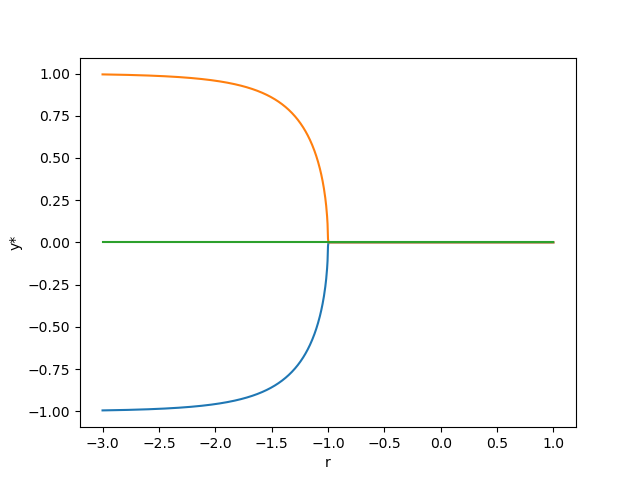
\includegraphics[width=\linewidth]{bifurcation_plot.png}
    \caption{Ruhelagen in Abhängigkeit von $r$}
\end{figure}
\end{solution}
